\documentclass[a4paper, 12pt]{article}

\usepackage{mathtools}
\usepackage{graphicx}
\usepackage{amsmath}

\usepackage{caption}
\usepackage{subcaption}

\usepackage[margin=1in, bottom=0.5in, includefoot]{geometry}

\usepackage{fancyhdr}
\pagestyle{fancy}
\fancyhead{}
\fancyfoot{}
\fancyfoot[R]{\thepage}
\renewcommand{\headrulewidth}{0pt}

\graphicspath{{./images/}}

\begin{document}

\begin{titlepage}
	\begin{center}
	
\includegraphics{logo}\\
	\large{\textbf{TRIBHUVAN UNIVERSITY\\ INSTITUTE OF ENGINEERING \\ PULCHOWK CAMPUS}}\\
	\large{LAB REPORT}\\
	
	\begin{picture}(50,250)
		\put(0,--25){\line(0,1){150}}
		\put(25,-25){\line(0,1){250}}
		\put(50,25){\line(0,1){150}}
	\end{picture}
	\end{center}
	\vspace{1cm}
	\begin{minipage}{2.5in}

    	Lab No: 1\\
    	Experiment Date: 2021-05-11\\
    	Submission Date: 2021-05-18\\

    	\textbf{\underline{Submitted By:}}\\
    	Name: Suban Shrestha \\
    	Roll No: 076BCT082 \\
    	Group: CD(D)
	\end{minipage}
	\hfill
	\begin{minipage}{1.3in}
    	\textbf{\underline{Submitted To:}}\\
    	Department of Electronics and Communications Enginnering
	\end{minipage}
\end{titlepage}

{\LARGE{\textbf{Basic Gates: AND, OR, NOT Gates; Universal  Gates: NAND, NOR Gates and XOR, XNOR Gates truth verifications.}}}
\section{Objectives}
\begin{itemize}
  \item
    To investigave differents gates.
  \item
    Veriy the truth table of the different gates.
  \item
    Construction and verification of three input AND gate using two input AND gate
  \item
    Construction and verification of four input OR gate using two input OR gates.
  \item
    To connenct interter gates in series in odd numbers and even numbers and observe thir property.
\end{itemize}

\section{Theory}
Logic gates are the basic building blocks of any digital system. Logic gate is an electronic circuit having one or more than one input and only one output. The relationship between the input and the ouput is based on a certain logic. \\
Logic gates perform some primary boolean operations and by combining various different logic gates, complex boolean functions can be implemented.


\subsection{AND Gate}
A gate that performs the logical AND operation is called AND Gate.It takes two or more inputs. The output of AND gate is high only when all the inputs are high. The logic is represented by dot(.) sign. For two inputs A and B, the output is written as $Y = A.B$.

\begin{minipage}[c]{.5\textwidth}
  \centering
    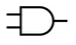
\includegraphics{and-gate}
    \captionof{figure}{AND Gate}
\end{minipage}
\begin{minipage}{.5\textwidth}
  \begin{center}
    \begin{tabular}{ |c|c|c| }
      \hline
      A & B & $Y = A.B$ \\
      \hline
      0 & 0 & 0 \\
      \hline
      0 & 1 & 0 \\
      \hline
      1 & 0 & 0 \\
      \hline
      1 & 1 & 1 \\
      \hline
    \end{tabular}
    \captionof{table}{Truth Table}
  \end{center}
\end{minipage}


\subsection{OR Gate}
A gate that performs the logical OR operation is called OR Gate. It takes two or more inputs. The output of OR gate is high when any one of the inputs is high. The logic is represented by plus(+) sign. For two inputs A and B, the output is written as $Y = A + B$.

\begin{minipage}[c]{.5\textwidth}
  \centering
    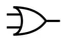
\includegraphics{or-gate}
    \captionof{figure}{OR Gate}
\end{minipage}
\begin{minipage}{.5\textwidth}
  \begin{center}
    \begin{tabular}{ |c|c|c| }
      \hline
      A & B & $Y = A+B$ \\
      \hline
      0 & 0 & 0 \\
      \hline
      0 & 1 & 1 \\
      \hline
      1 & 0 & 1 \\
      \hline
      1 & 1 & 1 \\
      \hline
    \end{tabular}
    \captionof{table}{Truth Table}
  \end{center}
\end{minipage}



\subsection{NOT Gate}
A gate that performs the logical NOT operation is called NOT Gate. The output of NOT gate is high when the input is low and ouput is low when the input is high. It is a single input gate. The logic is represented by a complement symbol('). For a input A, the output is written as $Y = A'$

\begin{minipage}[c]{.5\textwidth}
  \centering
    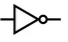
\includegraphics{not-gate}
    \captionof{figure}{NOT Gate}
\end{minipage}
\begin{minipage}{.5\textwidth}
  \begin{center}
    \begin{tabular}{ |c|c| }
      \hline
      A & $Y = A'$ \\
      \hline
      0 &  1 \\
      \hline
      1 &  0 \\
      \hline
    \end{tabular}
    \captionof{table}{Truth Table}
  \end{center}
\end{minipage}


\subsection{NAND Gate}
A gate that performs the logical AND followed by NOT operation is called NAND Gate. It takes two or more inputs and gives one output. The output is high when any one of the input is low. It is one of the universal gates. For two inputs A and B, the output is written as $Y = (A.B)'$.

\begin{minipage}[c]{.5\textwidth}
  \centering
    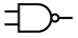
\includegraphics{nand-gate}
    \captionof{figure}{NAND Gate}
\end{minipage}
\begin{minipage}{.5\textwidth}
  \begin{center}
    \begin{tabular}{ |c|c|c| }
      \hline
      A & B & $Y = (A.B)'$ \\
      \hline
      0 & 0 & 1 \\
      \hline
      0 & 1 & 1 \\
      \hline
      1 & 0 & 1 \\
      \hline
      1 & 1 & 0 \\
      \hline
    \end{tabular}
    \captionof{table}{Truth Table}
  \end{center}
\end{minipage}


\subsection{NOR Gate}
A gate that perform the logical OR followed by NOT operation is called NOR Gate. It takes in two or more inputs and gives one output. The output is high only when none of the inputs are high. It is one of the universal gates. For two inputs A and B, the output is written as $Y = (A + B)'$

\begin{minipage}[c]{.5\textwidth}
  \centering
    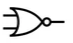
\includegraphics{nor-gate}
    \captionof{figure}{NOR Gate}
\end{minipage}
\begin{minipage}{.5\textwidth}
  \begin{center}
    \begin{tabular}{ |c|c|c| }
      \hline
      A & B & $Y=(A + B)'$ \\
      \hline
      0 & 0 & 1 \\
      \hline
      0 & 1 & 0 \\
      \hline
      1 & 0 & 0 \\
      \hline
      1 & 1 & 0 \\
      \hline
    \end{tabular}
    \captionof{table}{Truth Table}
  \end{center}
\end{minipage}


\subsection{XOR Gate}
Xor gate is a special type of gate. It performs the exclusive or operation of the input. It is also known as the even parity as the output is high only only when odd number of inputs are high. For two inputs A and B, the output is written as $Y = A \oplus B$.

\begin{minipage}[c]{.5\textwidth}
  \centering
    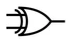
\includegraphics{xor-gate}
    \captionof{figure}{XOR Gate}
\end{minipage}
\begin{minipage}{.5\textwidth}
  \begin{center}
    \begin{tabular}{ |c|c|c| }
      \hline
      A & B & $Y=A\oplus B$ \\
      \hline
      0 & 0 & 0 \\
      \hline
      0 & 1 & 1 \\
      \hline
      1 & 0 & 1 \\
      \hline
      1 & 1 & 0 \\
      \hline
    \end{tabular}
    \captionof{table}{Truth Table}
  \end{center}
\end{minipage}


\subsection{XNOR Gate}
XNOR is a special type of gate. It perfroms the exclusive nor operation on the input. It is also knows as odd parity as the ouput is high only when even number of inputs are high. For two inputs A and B, the output is written as $Y = (A \oplus B)' $.
\begin{minipage}[c]{.5\textwidth}
  \centering
    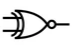
\includegraphics{xnor-gate}
    \captionof{figure}{XNOR Gate}
\end{minipage}
\begin{minipage}{.5\textwidth}
  \begin{center}
    \begin{tabular}{ |c|c|c| }
      \hline
      A & B & $Y=(A\oplus B)'$ \\
      \hline
      0 & 0 & 1 \\
      \hline
      0 & 1 & 0 \\
      \hline
      1 & 0 & 0 \\
      \hline
      1 & 1 & 1 \\
      \hline
    \end{tabular}
    \captionof{table}{Truth Table}
  \end{center}
\end{minipage}


\pagebreak
\section{Lab}
\subsection{Materials Required}
\begin{enumerate}
  \item
    And Gate
  \item
    Or Gate
  \item
    Not Gate
  \item
    Nand Gate
  \item
    Nor Gate
  \item
    Xor Gate 
  \item
    Xnor Gate 
  \item 
    Logic probes
  \item
    Logic State
  \item
    Proteus
\end{enumerate}

\subsection{Observations}

\subsubsection{AND gate}
A AND gate was connection to logic probe and logic states and its behaviour was observed.
The circuit and truth table obtained are listen below. \\

\begin{minipage}[c]{.7\textwidth}
  \centering
  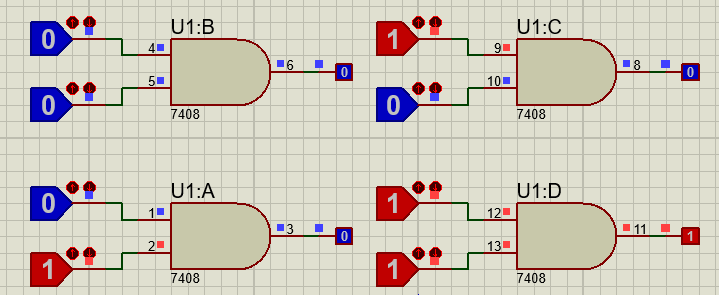
\includegraphics[scale=0.5]{and}
    \captionof{figure}{AND Gate}
\end{minipage}
\begin{minipage}{.3\textwidth}
  \begin{center}
    \begin{tabular}{ |c|c|c| }
      \hline
      A & B & $Y=A.B$ \\
      \hline
      0 & 0 & 0 \\
      \hline
      0 & 1 & 0 \\
      \hline
      1 & 0 & 0 \\
      \hline
      1 & 1 & 1 \\
      \hline
    \end{tabular}
    \captionof{table}{Truth Table}
  \end{center}
\end{minipage}

\subsubsection{3 Input AND Gate}
A 3 input AND gate can be constructed by using two and gates. In a 3 input AND gate, the output is high only when all 3 inputs are high.

\begin{minipage}[c]{.5\textwidth}
  \centering
  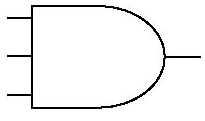
\includegraphics[scale=0.5]{3-input-and-gate}
    \captionof{figure}{3 Input AND Gate}
\end{minipage}
\begin{minipage}{.5\textwidth}
  \begin{center}
    \begin{tabular}{ |c|c|c|c| }
      \hline
      A & B & C & $Y = A.B.C$ \\
      \hline
      0 & 0 & 0 & 0 \\
      \hline
      0 & 0 & 1 & 0 \\
      \hline
      0 & 1 & 0 & 0 \\
      \hline
      0 & 1 & 1 & 0 \\
      \hline
      1 & 0 & 0 & 0 \\
      \hline 
      1 & 0 & 1 & 0 \\
      \hline
      1 & 1 & 0 & 0 \\
      \hline
      1 & 1 & 1 & 1 \\
      \hline
    \end{tabular}
    \captionof{table}{Truth Table}
  \end{center}
\end{minipage}

\begin{centering}
  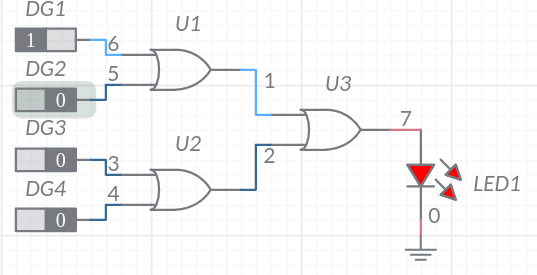
\includegraphics[scale=0.5]{4-input-or}
\captionof{figure}{4 Input OR}
\end{centering}



\subsubsection{OR gate}
A OR gate was connection to logic probe and logic states and its behaviour was observed.
The circuit and truth table obtained are listen below. \\

\begin{minipage}[c]{.7\textwidth}
  \centering
  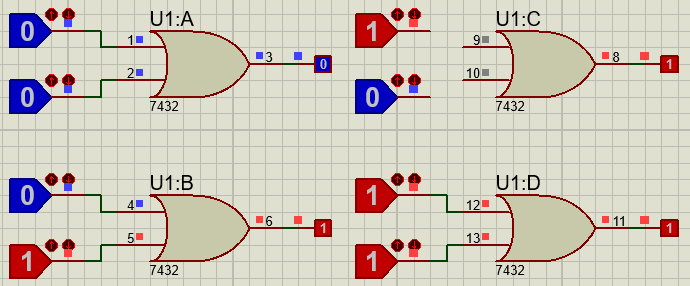
\includegraphics[scale=0.5]{or}
    \captionof{figure}{OR Gate}
\end{minipage}
\begin{minipage}{.3\textwidth}
  \begin{center}
    \begin{tabular}{ |c|c|c| }
      \hline
      A & B & $Y=A+B$ \\
      \hline
      0 & 0 & 0 \\
      \hline
      0 & 1 & 1 \\
      \hline
      1 & 0 & 1 \\
      \hline
      1 & 1 & 1 \\
      \hline
    \end{tabular}
    \captionof{table}{Truth Table}
  \end{center}
\end{minipage}

\subsubsection{4 Input OR Gate}
A 4 input OR gate can be constructed using three 2 input OR Gates. The output of the gate is high when any one of the inputs is high.

\begin{minipage}[c]{.5\textwidth}
  \centering
    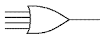
\includegraphics{4-input-or-gate}
    \captionof{figure}{4 Input OR Gate}
\end{minipage}
\begin{minipage}{.5\textwidth}
  \begin{center}
    \begin{tabular}{ |c|c|c|c|c| }
      \hline
      A & B & C & D & $Y = A+B+C+D$ \\
      \hline
      0 & 0 & 0 & 0 & 0 \\
      \hline
      0 & 0 & 0 & 1 & 1 \\
      \hline
      0 & 0 & 1 & 0 & 1 \\
      \hline
      0 & 0 & 1 & 1 & 1 \\
      \hline
      0 & 1 & 0 & 0 & 1 \\
      \hline
      0 & 1 & 0 & 1 & 1 \\
      \hline
      0 & 1 & 1 & 0 & 1 \\
      \hline
      0 & 1 & 1 & 1 & 1 \\
      \hline
      1 & 0 & 0 & 0 & 1 \\
      \hline
      1 & 0 & 0 & 1 & 1 \\
      \hline
      1 & 0 & 1 & 0 & 1 \\
      \hline
      1 & 0 & 1 & 1 & 1 \\
      \hline
      1 & 1 & 0 & 0 & 1 \\
      \hline
      1 & 1 & 0 & 1 & 1 \\
      \hline
      1 & 1 & 1 & 0 & 1 \\
      \hline
      1 & 1 & 1 & 1 & 1 \\
      \hline
    \end{tabular}
    \captionof{table}{Truth Table}
  \end{center}
\end{minipage}

\begin{centering}
  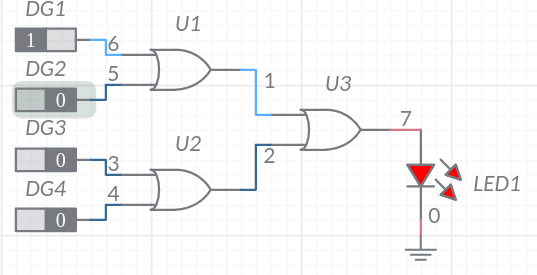
\includegraphics[scale=0.5]{4-input-or}
\captionof{figure}{4 Input OR}
\end{centering}

\subsubsection{NOT gate}
A NOT gate was connection to logic probe and logic states and its behaviour was observed.
The circuit and truth table obtained are listen below. \\

\begin{minipage}[c]{.7\textwidth}
  \centering
  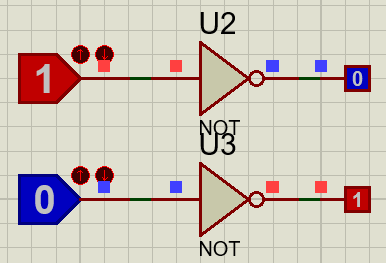
\includegraphics[scale=0.5]{not}
    \captionof{figure}{NOT Gate}
\end{minipage}
\begin{minipage}{.3\textwidth}
  \begin{center}
    \begin{tabular}{ |c|c| }
      \hline
      A &  $Y=A'$ \\
      \hline
      0 & 1 \\
      \hline
      1 & 0 \\
      \hline
    \end{tabular}
    \captionof{table}{Truth Table}
  \end{center}
\end{minipage}


\subsubsection{NAND gate}
A NAND gate was connection to logic probe and logic states and its behaviour was observed.
The circuit and truth table obtained are listen below. \\

\begin{minipage}[c]{.7\textwidth}
  \centering
  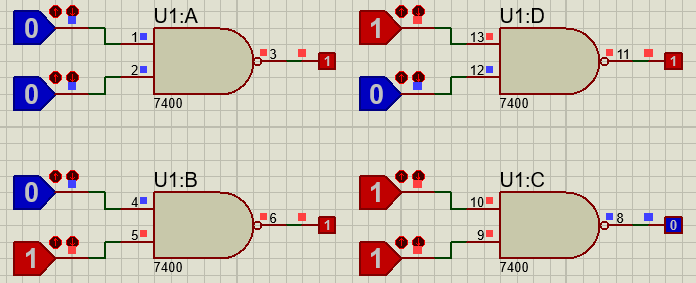
\includegraphics[scale=0.5]{nand}
    \captionof{figure}{NAND Gate}
\end{minipage}
\begin{minipage}{.3\textwidth}
  \begin{center}
    \begin{tabular}{ |c|c|c| }
      \hline
      A & B & $Y=(A.B)'$ \\
      \hline
      0 & 0 & 1 \\
      \hline
      0 & 1 & 0 \\
      \hline
      1 & 0 & 0 \\
      \hline
      1 & 1 & 0 \\
      \hline
    \end{tabular}
    \captionof{table}{Truth Table}
  \end{center}
\end{minipage}


\subsubsection{NOR gate}
A NOR gate was connection to logic probe and logic states and its behaviour was observed.
The circuit and truth table obtained are listen below. \\

\begin{minipage}[c]{.7\textwidth}
  \centering
  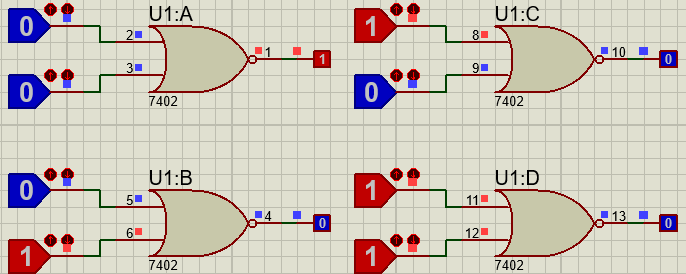
\includegraphics[scale=0.5]{nor}
    \captionof{figure}{NOR Gate}
\end{minipage}
\begin{minipage}{.3\textwidth}
  \begin{center}
    \begin{tabular}{ |c|c|c| }
      \hline
      A & B & $Y=(A+B)'$ \\
      \hline
      0 & 0 & 1 \\
      \hline
      0 & 1 & 1 \\
      \hline
      1 & 0 & 1 \\
      \hline
      1 & 1 & 0 \\
      \hline
    \end{tabular}
    \captionof{table}{Truth Table}
  \end{center}
\end{minipage}


\subsubsection{XOR gate}
A XOR gate was connection to logic probe and logic states and its behaviour was observed.
The circuit and truth table obtained are listen below. \\

\begin{minipage}[c]{.7\textwidth}
  \centering
  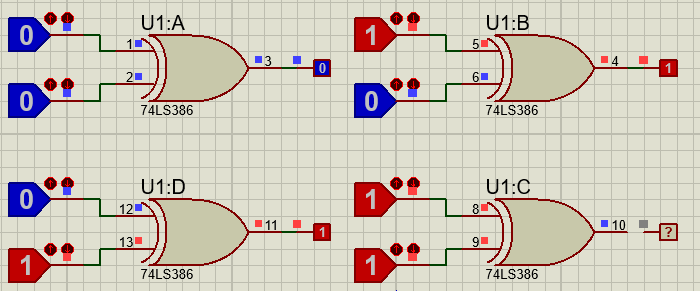
\includegraphics[scale=0.5]{xor}
    \captionof{figure}{XOR Gate}
\end{minipage}
\begin{minipage}{.3\textwidth}
  \begin{center}
    \begin{tabular}{ |c|c|c| }
      \hline
      A & B & $Y=A\oplus B$ \\
      \hline
      0 & 0 & 0 \\
      \hline
      0 & 1 & 1 \\
      \hline
      1 & 0 & 1 \\
      \hline
      1 & 1 & 0 \\
      \hline
    \end{tabular}
    \captionof{table}{Truth Table}
  \end{center}
\end{minipage}


\subsubsection{XNOR gate}
A XNOR gate was connection to logic probe and logic states and its behaviour was observed.
The circuit and truth table obtained are listen below. \\

\begin{minipage}[c]{.7\textwidth}
  \centering
  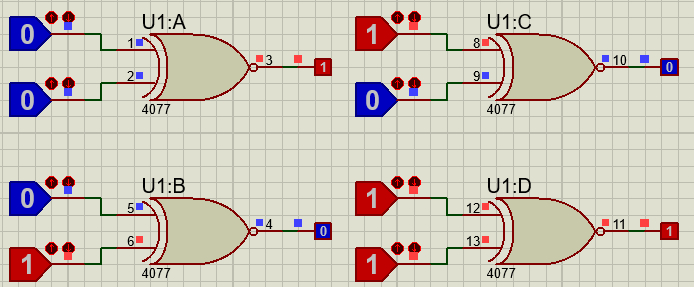
\includegraphics[scale=0.5]{xnor}
    \captionof{figure}{XNOR Gate}
\end{minipage}
\begin{minipage}{.3\textwidth}
  \begin{center}
    \begin{tabular}{ |c|c|c| }
      \hline
      A & B & $Y=(A\oplus B)'$ \\
      \hline
      0 & 0 & 1 \\
      \hline
      0 & 1 & 0 \\
      \hline
      1 & 0 & 0 \\
      \hline
      1 & 1 & 1 \\
      \hline
    \end{tabular}
    \captionof{table}{Truth Table}
  \end{center}
\end{minipage}

\subsection{Realization of gates using Universal Gates}

\subsubsection{NAND gate}

\begin{centering}
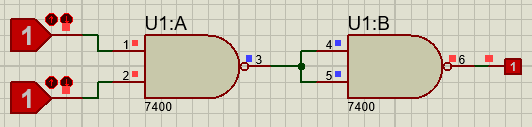
\includegraphics{nand-and}
\captionof{figure}{AND from NAND Gate}
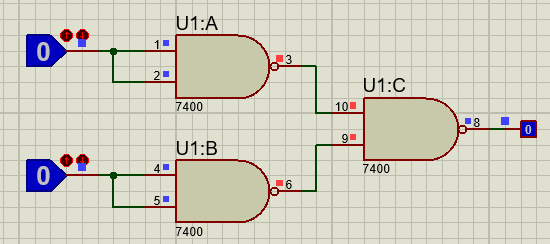
\includegraphics[scale=0.5]{nand-or}
\captionof{figure}{or from NAND Gate}
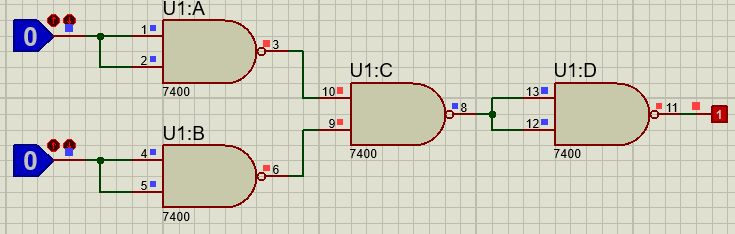
\includegraphics[scale=0.5]{nand-nor}
\captionof{figure}{nor from NAND Gate}
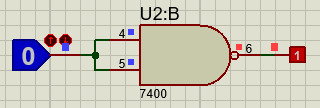
\includegraphics{nand-not}
\captionof{figure}{NOT from NAND Gate}
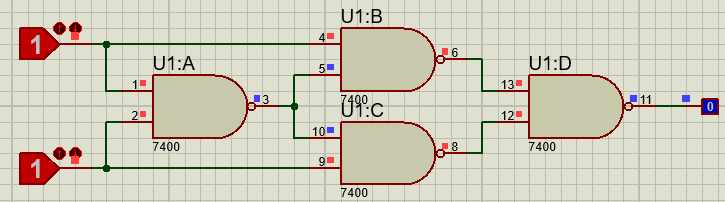
\includegraphics[scale=0.5]{nand-xor}
\captionof{figure}{XOR from NAND Gate}
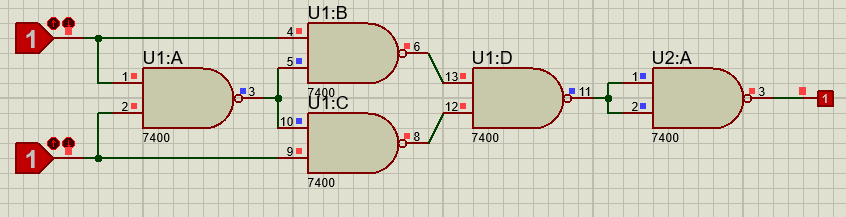
\includegraphics[scale=0.5]{nand-xnor}
\captionof{figure}{XNOR from NAND Gate}
\end{centering}

\subsubsection{NOR gate}
\begin{centering}
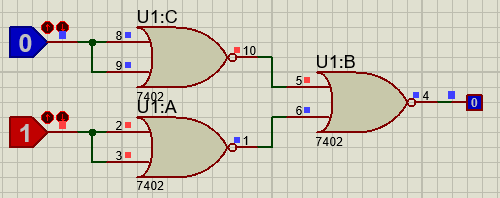
\includegraphics{nor-and}
\captionof{figure}{AND from NOR Gate}
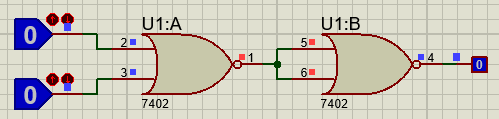
\includegraphics[scale=0.5]{nor-or}
\captionof{figure}{OR from NOR Gate}
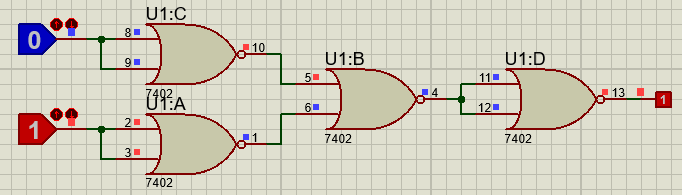
\includegraphics[scale=0.5]{nor-nand}
\captionof{figure}{NAND from NOR Gate}
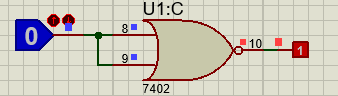
\includegraphics{nor-not}
\captionof{figure}{NOT from NOR Gate}
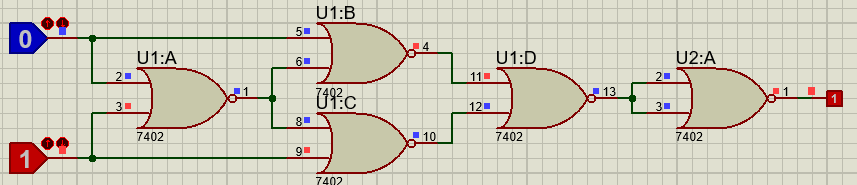
\includegraphics[scale=0.5]{nor-xor}
\captionof{figure}{XOR from NOR Gate}
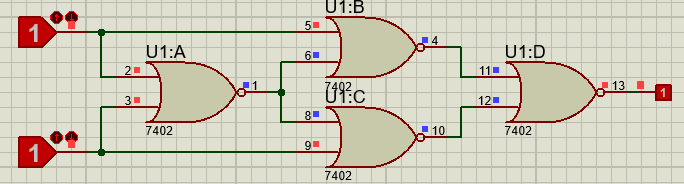
\includegraphics[scale=0.5]{nor-xnor}
\captionof{figure}{XNOR from NOR Gate}
\end{centering}



\pagebreak
\section{Discussion}
The inputs and outputs of AND, OR, NOT, NOR, NAND, XOR and XNOR gates, their symbols and truth tables were studied. Then proteus was used to realize the gates and their respective truth tables were verified. The working of 3 input AND gate and 4 input OR gate was also studied. The theory behind the universal gates was also studied and they were used to make other gates. 


\section{Conclusion}
Thus a concise understanding of various logic gates was obtained, my closely studying their behaviour, symbols, and their truth tables. And proteus was used for the verification of their truth tables. 3 input AND gate and 4 input OR gate was also studied. And the universal gates were used to construct other gates.

\end{document}

